%----------------------------------------------------------------------------
\chapter{Test design and documentation}\label{chapter:TestDoc}
%----------------------------------------------------------------------------
\section{Test design techniques}

The MoDeS$^3$ is a multi-layered, safety-critical application, which consist of off-the-self and custom made components also. As a complex system it is crucial to have a well-designed testing process and documentation which helps determine any problem in the system. For this purpose in the following chapter I will examine the possible and most suitable test approaches.

\begin{figure}[!h]
	\centering
	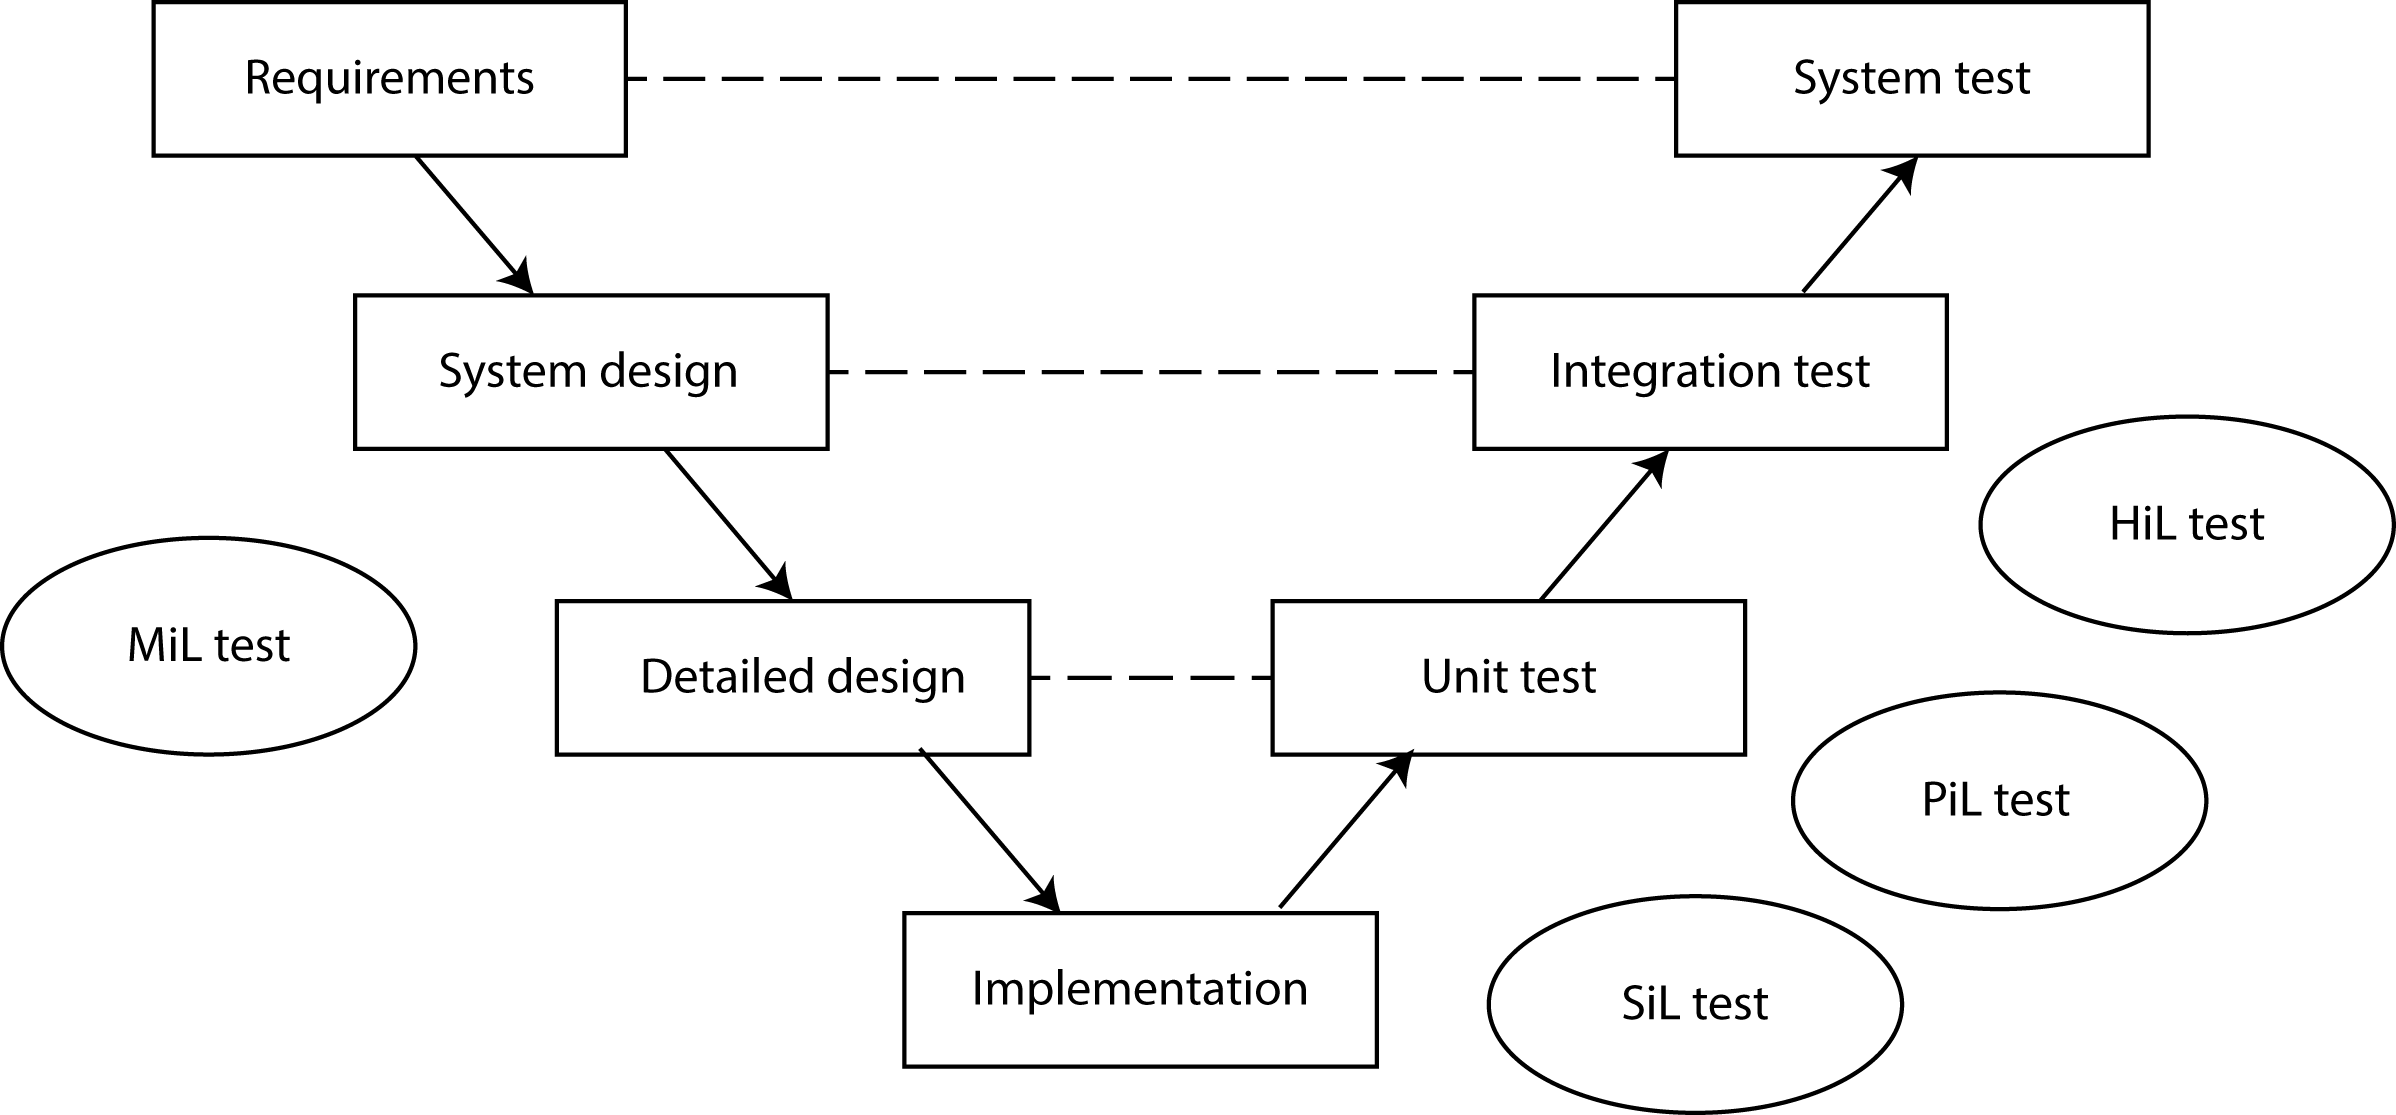
\includegraphics[width=150mm]{figures/testDesign/V_model1.png}
	\caption{V-model levels overview. Adapted from \cite{Vmodel}}
	\label{fig:vModel}
\end{figure}

\subsection{V-model and testing levels}
Nowadays one of the most popular software development methodology is the V-model \cite{Vmodel} (shown on figure \ref{fig:vModel}), which defines four stages during the development and four verification steps accordingly (each step is shown with rectangles on the figure). In addition for making the development more effective for error-detection, there are four more steps defined for verifying our system's correctness, called test levels \cite{TestLevels} (shown with ellipses). While the development starts with an abstract \textbf{requirement analysis}, which declares the aim of our application, later on each step contains more detailed information. The second phase is about understanding the abstract user requirements and define the system's \textbf{functional specification} by the developers. During this phase our verification is based on \textbf{Model-in-the-Loop (MiL) testing}. The third phase contains all the low-level design and specific information about the application. From these design decisions, the \textbf{implementation} should be quite straight-forward or even it can be generated. During the \textbf{Software-in-the-Loop (SiL) testing}, the implementation will be verified for a subset of functionalities, which is depending on the system's purpose and requirements.
As of now our implementation is done and our design decisions are verified, we make sure with \textbf{unit tests} that our functions are serving their exact purposes. \textbf{Processor-in-the-Loop (PiL)} testing ensures that the computing processor at the bottom of the V-model works as expected. Then moving up in the V-model with \textbf{integration tests}, we are focusing on more abstract and complex components. In this phase we consider software and hardware elements also, completed with \textbf{Hardware-in-the-Loop (HiL)} testing. The last step is about verifying the complete system in real environment and check the high-level requirements.

\subsection{Specification-based testing techniques}
During the test design process and implementation phases, the conception can be a quite complex and difficult task. Nevertheless the test design techniques can be useful in these situations. The commonly used approaches are described in this section, which are used during the MoDeS$^3$ test design process, based on \cite{IEEE13}. These methods can be divided into 3 branches, which are specification-based, structure-based and experience-based techniques. The first is deriving the tests from the system specification details. In opposite to that the structure-based approach is based on the system architecture (in software systems the implementation architecture). The third branch is a way to test a system, which is lack of structure and specification documentation. 

The following paragraphs are details 3 design technique, which are belongs to the specification-based area.
\paragraph{Scenario Testing} The first technique is consists of specifying the interactions between the test items and the intervened system, which is usually a user. Therefore this technique is also called use-case testing. 

\paragraph{Equivalence Class Partitioning} The key point in the equivalence class partitioning is to categorize the test item inputs and outputs into classes, which are similar in these aspects. In addition these partitions can cover valid and invalid inputs or outputs also. 

\paragraph{Decision Table Testing} If the test items can be identified with a logical relationship between the input and output values where these values can have only 2 partitions, then during the test design the decision table testing can be used.

\section{Test documentation}
During the test design phases of the MoDeS$^3$ I will follow a subset of the ISO 291119 standard \cite{IEEE13}.
First this section describes the documents in general, which will be later used in the MoDeS$^3$ test documentation process in section \autoref{TestDoc:MODES}. As of now the organizational and role details are irrelevant for this project, I will just give a short example for those. In the following sections, I will subtract the documentations into 3 phases, called Organizational, Test Management and Dynamic Test Documentation. 

\begin{figure}[!h]
	\centering
	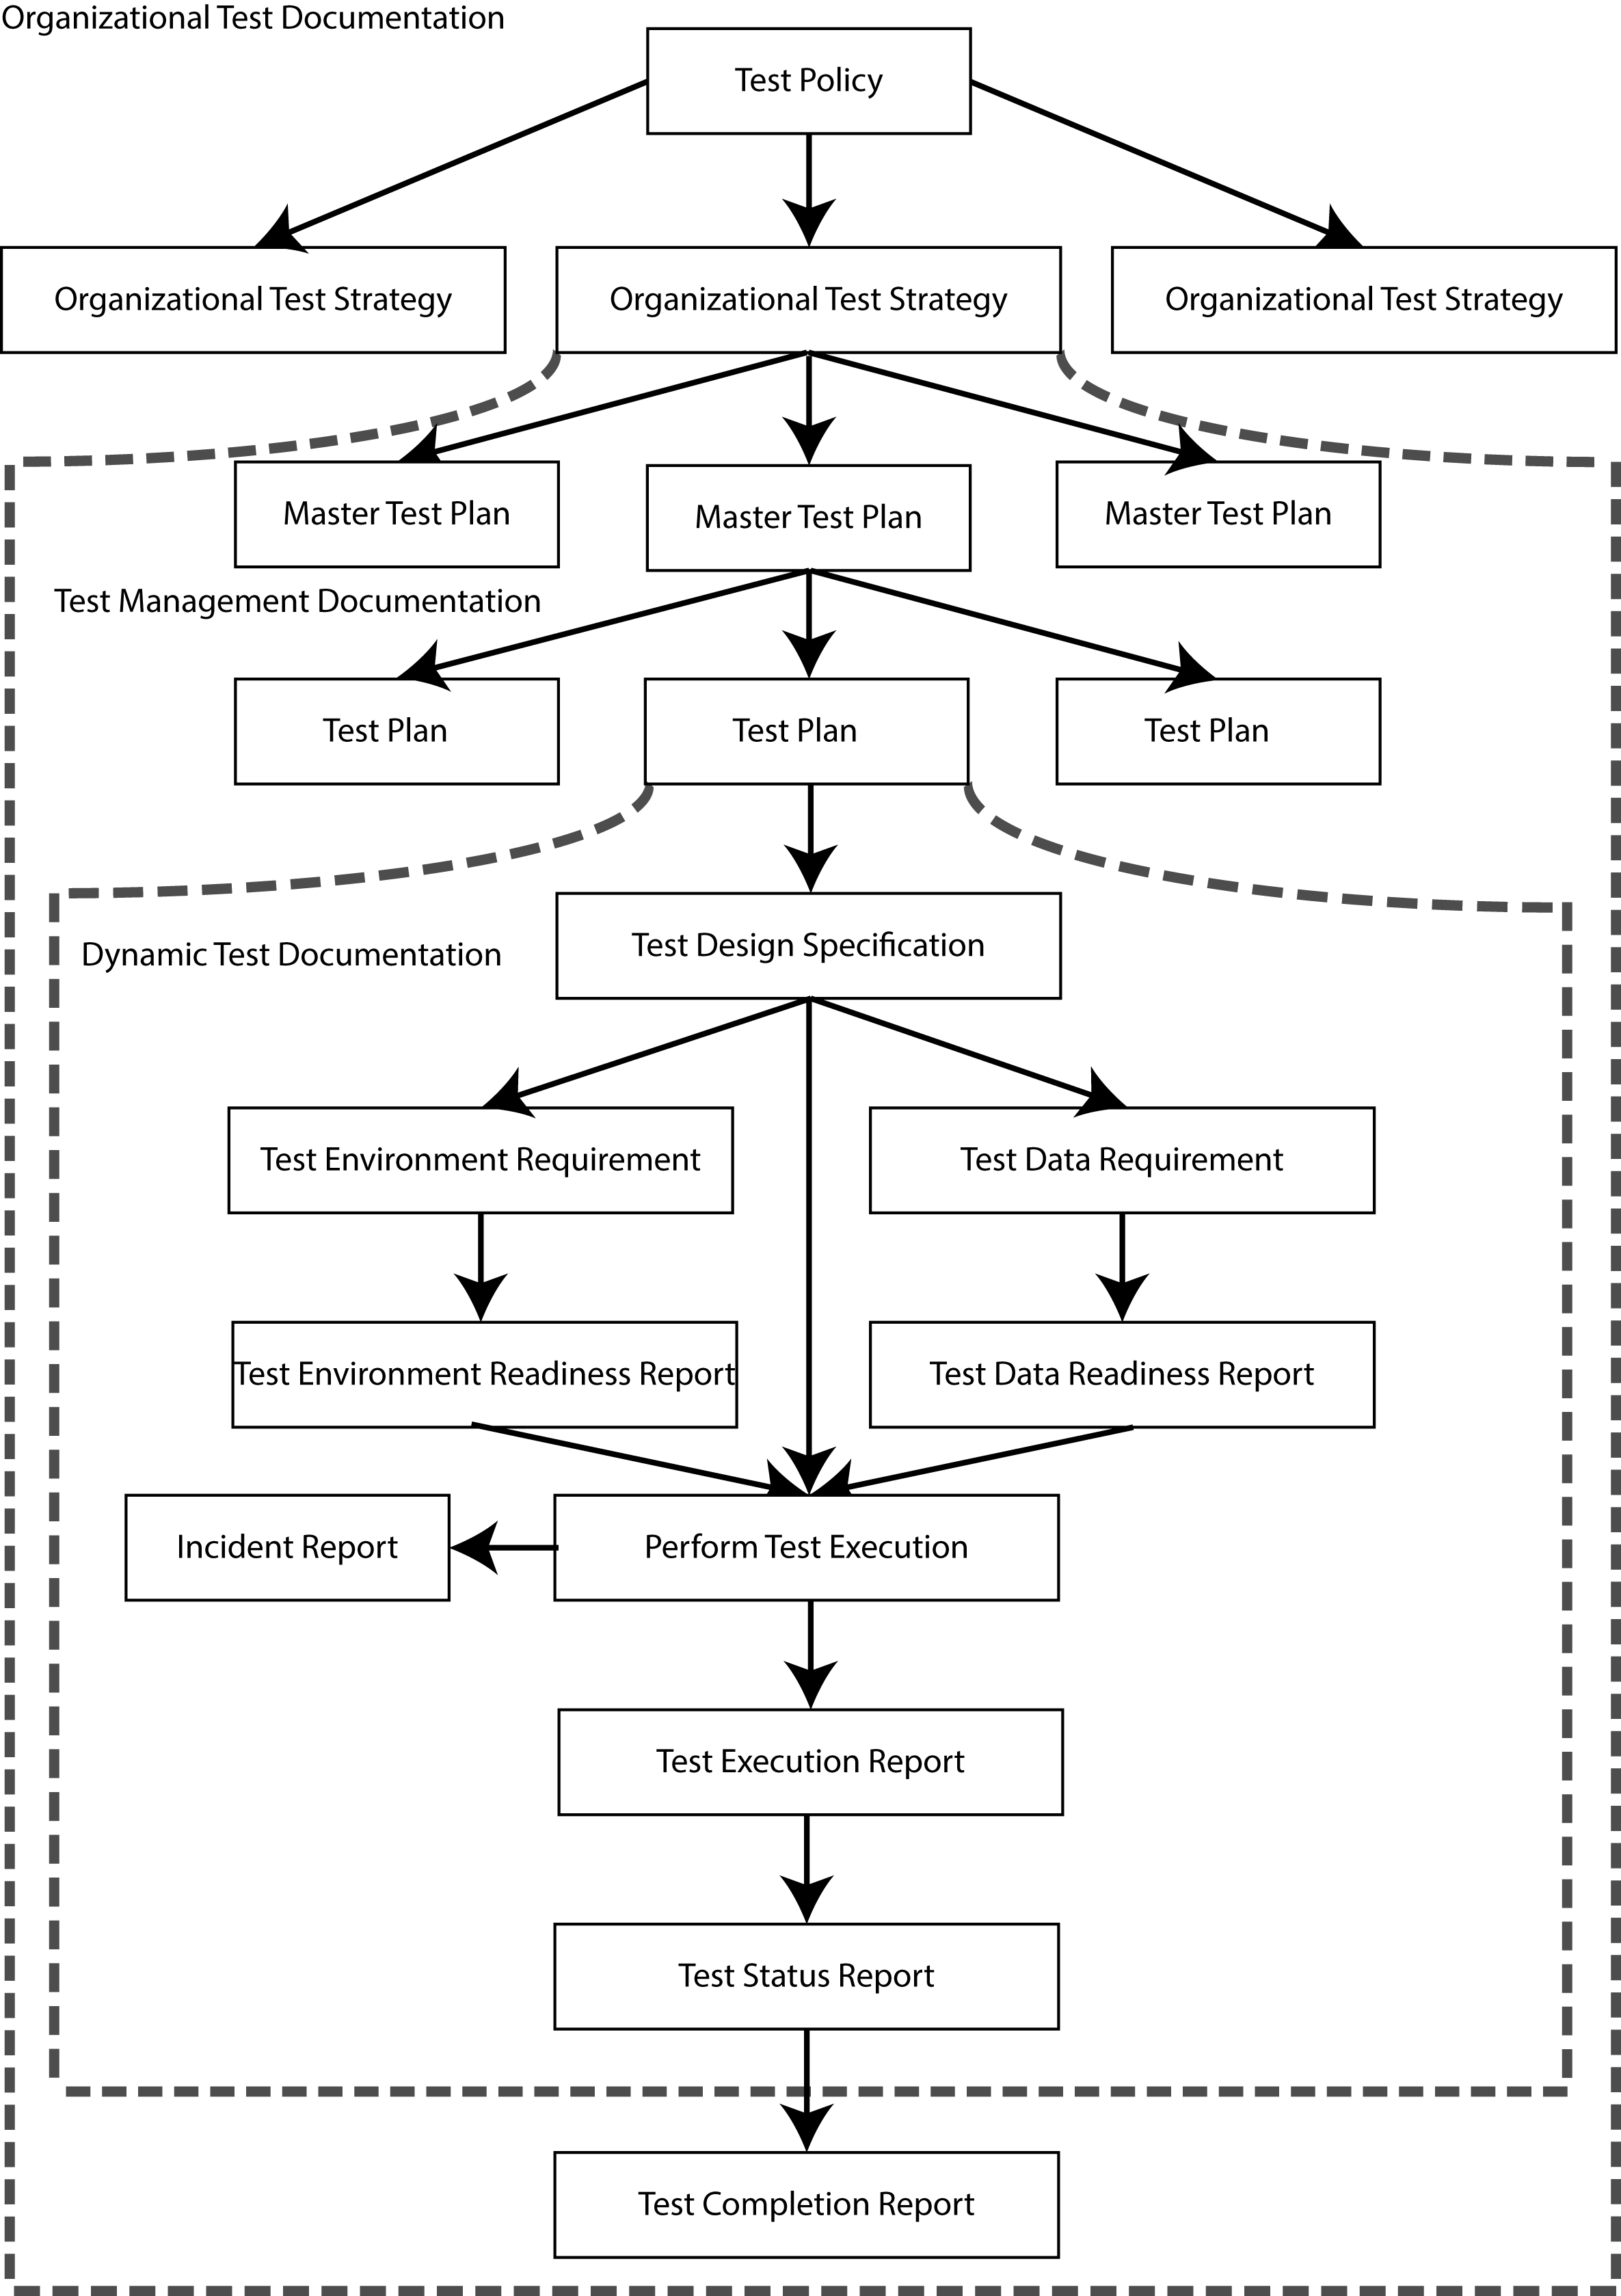
\includegraphics[width=150mm, keepaspectratio]{figures/testDesign/TestDoc1.png}
	\caption{Test Documentation Overview. Adapted from \cite{IEEE13}}
	\label{fig:TestDocOverview}
\end{figure}

\subsection{Organizational test documentation}
These general documents must be distributed organizational-wise and must be the same for every project within the organization. In according to this, during the test documentation the organization will be the MoDeS$^3$ team and the only project will be the above detailed railway system.

\paragraph{Test Policy}
Throughout the test development a Test Policy must contain the test principles and objectives for the whole organization. It clarifies what should be tested during development, but not how testing must be implemented. Furthermore it must define the provisions to be used for establishing, improving, maintaining and reviewing the test Policy.

\paragraph{Test Strategy}
A Test Strategy must define a proper guideline on how testing should be performed for all projects in the organization. In our case one Test Strategy is sufficient, but for an organization which have projects in different technical areas, can have a Test Strategy for each area. In latter case, the organization can define separate Test sub-processes to satisfy any special need for an area or project.

%\begin{enumerate}
%	\item Organizational Test Strategy
%	\begin{enumerate}
%		\item Introduction
%		\item General test strategy statements
%		\begin{enumerate}
%			\item Generic risk management
%			\item Test selection and prioritization
%			\item Test documentation and reporting
%			\item Test automation and tools
%			\item Configuration management of test work products
%			\item Incident management
%			\item Test sub-processes
%		\end{enumerate}
%	\end{enumerate}
%\end{enumerate}

\subsection{Test Management Documentation}
The Test Management Documentation is focusing on one project's planning and test evaluation. This group of documentation provides guidelines for Test Plan, Test Status Report and Test Completion Report.

\paragraph{Test Plan}
The collection of the test planning and test management documents is the Test Plan. It's scope be mapped to multiple projects, a single project or to sub-projects, where each Test Plan is dedicated for a sub-process (For example system test plan, integration software test plan, sub-system test plan, or unit software test plan). In a complex design structure it is advised to have a mapping tree document, which shows the relations between these Test Plans.

\paragraph{Test Status Report}
A report from the currently ongoing test process in a given reporting period is the Test Status Report. For example in an agile project it can be delivered at the end of the iteration. Although it is not necessarily a written document.

\paragraph{Test Completion Report}
As a summary of our test execution, a Test Completion Report can be provided for every test sub-process or for the whole project itself.

\subsection{Dynamic Test Documentation}
During the Dynamic Test Documentation phase the following documents are prepared:
\begin{itemize}
	\item Test Specification with sub-documents of:
	\begin{itemize}
		\item Test Design Specification
		\item Test Case Specification
		\item Test Procedure Specification
	\end{itemize}
	\item Test Data Requirements
	\item Test Environment Requirements
	\item Test Data Readiness Report
	\item Test Environment Readiness Report
	\item Test Execution Documentation with sub-documents of:
	\begin{itemize}
		\item Actual Result
		\item Test Results
		\item Test Execution Log
		\item Incident Report
	\end{itemize}
\end{itemize}

In the following sections, I will give a brief summary for each documentation.

\paragraph{Test Design Specification} \label{TestDoc:TDS}
The features and test conditions (derived from test basis) are collected in the Test Design Specification with the specific test cases and test procedures. These detailed test cases will be executed during testing process. 

Here we can create groups called \textit{feature sets} for those features which are connected together, then we can handle them independently.  A \textit{test condition} is aligned for each feature set and can be verified by a test case. Technically a test condition means a concrete state or representation of a feature. In addition on or more requirement can be referenced by a test case. In addition, to develop a more maintainable test document we must take care for the references from test cases to each requirement.

\paragraph{Test Case Specification}
One or more feature set with the defined test conditions and coverage items, constitutes a Test Case Specification.

\textit{Test coverage items} are obtained from a set of test conditions and specific test design technique. These items can be summarized in a list (describing test coverage items, test conditions and feature sets with proper priorities). From each test coverage item a \textit{Test case} can be derived, which verifies the correct implementation of a function. Regarding the possible number of test cases it can be collected into a list, table or database. Each test case should have a proper definition of dependencies. These are collected in \autoref{table:TestDoc:TestCases}.

\begin{table}[h]
	\caption{Details of a test case}
	\label{table:TestDoc:TestCases}
	\begin{center}
		\renewcommand{\arraystretch}{1.8}
		\begin{tabu} 
			to 0.9 \textwidth
			{  X[0.3, c]  X[c] }
			\toprule
			Aspect                     & Description                                                                                                                                               \\ \midrule
			Priority                   & Defines the execution order and importance between test cases. Higher priority test cases should be examined earlier then lower priorities                \\
			Traceability               & Reference the parent test coverage, condition item and the feature requirement                                                                            \\
			Preconditions              & Describes special states that must exists to execute the test case (Can be other test cases also)                                                         \\
			Inputs                     & A specific action which sets the test item into a state, where the actual and expected results can be compared                                            \\
			Expected result            & Specifies the expected output and behavior (with tolerances) of the test item which was in the precondition state and was modified with the proper inputs \\
			Actual result, test result & A description of test item outputs and a comparison between actual and expected results                                                                   \\ \bottomrule
		\end{tabu}
	\end{center}
\end{table} 

\paragraph{Test Procedure Specification}
Describes the precondition setup and test cases execution in the proper order with possible post evaluation activities.

Those test cases, which have the same purpose in the test item's property (for example precondition, test basis or even in the identified risk) can be collected into a \textit{Test set}. Typically this will reflect to one or more feature sets. For each \textit{Test set} the proper execution order is defined in the \textit{Test procedure} considering test case dependencies, preconditions, postconditions and other environment requirements.

\paragraph{Test Data Requirements}
Defines the required properties of the test data, which is used during test procedure execution. These requirements can be summarized with a list. In addition, this detailed test data requirements makes it more maintainable and traceable. 

\paragraph{Test Data Readiness Report} 
Gives a list of Test Data Requirements determining whether they are satisfied or not.

\paragraph{Test Environment Requirements}
Describes the required test environment properties, which are setting the test items into the expected test environment. These requirements can also be grouped by environment types like hardware, middleware, software, tools or security and may vary for each test case.

\paragraph{Test Environment Readiness Report}
Lists the fulfillment of Test Environment Requirements.

\paragraph{Actual Results and Test Results}
After executing the selected test procedures, each test case's actual result (output state or behavior after the input actions) should be recorded. It may require full recording of the process with an automated tool also. Each Test Result determines if the actual results are corresponding to the expected results with the specified deviation or not. It is usually recorded as passed or failed, along with the actual results.

\paragraph{Test Execution Report}
Detailed documentation of one or more test procedure's execution. Can be represented in a list or table with measuring times and events of the test execution.

\paragraph{Test Incident Report}
If there is any deviation between the actual and expected results after each test procedure execution, we should create a dedicated Incident Report detailing the problems. These reports could contain a description of the problem with severity, date and possible risk information.
